% Template for ISBI-2011 paper; to be used with:
%          spconf.sty  - ICASSP/ICIP LaTeX style file, and
%          IEEEbib.bst - IEEE bibliography style file.
% --------------------------------------------------------------------------
\documentclass{article}
\usepackage{spconf,amsmath,graphicx}
\graphicspath{{pdf/}{png/}}
\usepackage[printonlyused,nolist]{acronym}
\usepackage[colorlinks=true,linkcolor=black,citecolor=black]{hyperref}
\usepackage{colortbl}

% Example definitions.
% --------------------
\def\x{{\mathbf x}}
\def\L{{\cal L}}

% Title.
% ------
\title{An Analysis of Blood-Oxygen-Level-Dependent Signal Parameter Estimation Using Particle Filters}
%
% Single address.
% ---------------
\name{Chambers, Micah C}
\address{Virginia Tech\\
    Bradley Department of Electrical and Computer Engineering\\
    302 Whittemore Hall\\
    Blacksburg, VA 24061-0111}
%
% For example:
% ------------
%\address{School\\
%	Department\\
%	Address}
%
% Two addresses (uncomment and modify for two-address case).
% ----------------------------------------------------------
%\twoauthors
%  {A. Author-one, B. Author-two\sthanks{Thanks to XYZ agency for funding.}}
%	{School A-B\\
%	Department A-B\\
%	Address A-B}
%  {C. Author-three, D. Author-four\sthanks{The fourth author performed the work
%	while at ...}}
%	{School C-D\\
%	Department C-D\\
%	Address C-D}
%
% More than two addresses
% -----------------------
% \name{Author Name$^{\star \dagger}$ \qquad Author Name$^{\star}$ \qquad Author Name$^{\dagger}$}
%
% \address{$^{\star}$ Affiliation Number One \\
%     $^{\dagger}$}Affiliation Number Two
%


\begin{document}
%\ninept
%
\maketitle
%
\begin{abstract}
The Blood-Oxygen-Level-Dependent (BOLD) Signal that is measured by functional 
magnetic resonance imaging (fMRI)
has been the subject of extensive research since the first development 
of the balloon model. While there would be definite benefits to 
moving from the General Linear Model to a physiologically inspired
BOLD model, significant barriers remain. Optimizing even the simplest
balloon model requires searching in 7 dimensions, and even more flexible
models are available. Whereas traditional methods of analyzing fMRI asks
where activation occurs, BOLD models would ask what the activation 
looks like. Unfortunately, the nonlinear nature of the Balloon Model
makes it difficult to analyze, therefore this work demonstrates the 
use of a particle filter to regresses the simplest form of the BOLD 
model. The results show that the system of equations are not observable,
leading to a large range of valid model parameters. 
\end{abstract}
%
\begin{keywords}
BOLD Response, FMRI, Nonlinear Systems, Particle Filter, Bayesian Statistics, System Identification
\end{keywords}
%

\begin{acronym}[CMRO2]
\acro{BOLD}{Blood-Oxygen-Level-Dependent}
\acro{CBF}{Cerebral Blood Flow}
\acro{CBV}{Cerebral Blood Volume}
\acro{CMRO2}{Cerebral Metabolic Rate of Oxygen}
\acro{DC}{Direct Current}
\acro{dHb}{Deoxygenated Hemoglobin}
\acro{EM}{Expectation-Maximization}
\acro{EPI}{Echo Planar Imaging}
\acro{fMRI}{Functional Magnetic Resonance Imaging}
\acro{FMRIB}{Oxford Centre for Functional MRI of the Brain}
\acro{FSL}{FMRIB Software Library}
\acro{FWHM}{Full-Width Half-Maximum}
\acro{GA}{Genetic Algorithms}
\acro{GLM}{General Linear Model}
\acro{HRF}{Hemodynamic Response Function}
\acro{Hb}{Hemoglobin}
\acro{MAD}{Median Absolute Deviation}
\acro{MI}{Mutual Information}
\acro{MR}{Magnetic Resonance}
\acro{MRI}{Magnetic Resonance Imaging}
\acro{MSE}{Mean Squared Error}
\acro{O2Hb}{Oxygenated Hemoglobin}
\acro{ODE}{Ordinary Differential Equation}
\acro{PDF}{Probability Density Function}
\acro{POSSUM}{Physics-Oriented Simulated Scanner for Understanding MRI}
\acro{RF}{Radio Frequency}
\acro{RMSE}{Root Mean Squared Error}
\acro{RMSR}{Root Mean Squared Residual}
\acro{SA}{Simulated Annealing}
\acro{SNR}{Signal-to-Noise Ratio}
\acro{SPM}{Statistical Parametric Mapping}
\acro{T1}{Longitudinal}
\acro{T2}{Spin-Spin}
\acro{TR}{Repetition Time}
\acro{UKF}{Unscented Kalman Filter}
\end{acronym}
\section{Introduction}
\label{sec:intro}
Traditional methods of analyzing timeseries images produced by 
\ac{fMRI} perform regression using the linear combination of explanatory variables. 
Though moving to a state space model with more more degrees of freedom 
requires additional computation, in this paper Particle Filters will
be used to estimate the governing parameters of the \ac{BOLD} model 
at a computation cost 
that would still allow real time calculations for multiple voxels.
In practical terms, this algorithm could be used as an alternative to \ac{SPM}
for activation detection. Though more computationally intense,
this method is capable of modeling nonlinear effects
and provides more detailed output. 

In particular this work focuses
on the observability of the \ac{BOLD} state equations from Friston et al.
\cite{Friston2000}. Because of the nonlinearities in the state equations,
no analytical method exists to determine observability, however little
movement in parameters was necessary to achieve high predictive quality from a
set parameters. High correlation as calculated from the joint \ac{PDF}
also indicates a lack of observability.  Future works will benefit from
restricting parameters and thus reducing the dimensionality of the system.
While this could reduce the plausibility of parameter estimates, it would
allow for better differentiation of parameters for analyzing pathologies
and reduce reduce computation time from the 40 seconds of analysis
per 5 minute timeseries (on a Core 2 Duo Q6600).

\subsection{BOLD Model}
It is well known that the two types of \ac{Hb} act as contrast agents in 
\ac{EPI} imaging \cite{Buxton1998, WEISSKOFF1994, Ogawa}, however the connection
between \ac{dHb}/\ac{O2Hb} and neural activity is non-trivial. 
Intuitively, increased 
metabolism will increase \ac{dHb}, however blood vessels are quick
to compensate by increasing local blood flow. Increased inflow, accomplished by loosening 
capillary beds, precedes increased outflow, driving increased 
blood storage.
Since the local \ac{MR} signal depends on the ratio of \ac{dHb} to \ac{O2Hb},
increased blood volume affects this ratio if 
metabolism doesn't exactly match the increased inflow of oxygenated blood.
This was the impetus
for the ground breaking balloon model \cite{Buxton1998} and windkessel
model \cite{Mandeville1999}. These works derive, from first principals,
the changes in \ac{dHb} ratio and volume of capillaries given an inflow waveform.
These were the first two attempts to quantitatively account for the shape of the 
\ac{BOLD} signal as a consequence of the lag between the \ac{CBV}
and the inward \ac{CBF}. 

Although Buxton et al. demonstrated that a well chosen flow waveform could 
explain most features of the \ac{BOLD} signal, it stopped short of proposing a
realistic waveform for the \ac{CBF} and \ac{CMRO2} \cite{Buxton1998}. Friston et al. 
gave a reasonable and simple
expression for \ac{CBF} input based on a flow inducing signal
and in the same work proposed a simple method
of estimating metabolic rate: as a direct function of the inward blood flow \cite{Friston2000}.
By combining these equations with the balloon model from Buxton et al.,
it is possible to predict the \ac{BOLD} signal directly from a stimulus time course:
\begin{eqnarray}
\label{eq:bold1}
\dot{s} &=& \epsilon u(t) - \frac{s}{\tau_s} - \frac{f - 1}{\tau_f} \\
\label{eq:bold2}
\dot{f} &=& s\\
\label{eq:bold3}
\dot{v} &=& \frac{1}{\tau_0}(f - v^\alpha)\\
\label{eq:bold4}
\dot{q} &=& \frac{1}{\tau_0}(\frac{f(1-(1-E_0)^f)}{E_0} - \frac{q}{v^{1-1/\alpha}})
\end{eqnarray}
where $s$ is a flow inducing signal, $f$ is the input \ac{CBF},
$v$ is normalized \ac{CBV}, and $q$ is the normalized
local \ac{dHb} content. The 
parameters controlling blood flow are $\epsilon$, which is a neuronal 
efficiency term, $u(t)$ which is the stimulus, and $\tau_f$, $\tau_s$ 
which are time constants. The parameters for the evolution of blood 
volume are $E_0$ which the resting metabolic
rate and $\alpha$ which is Grubb's parameter controlling the balloon model. 
$\tau_0$ is a single time constant controlling the speed of $v$ and $q$.

Obata refined the readout equation 
of the \ac{BOLD} signal based on the
\ac{dHb} content (q) and local blood volume (v), resulting in the
final \ac{BOLD} measurement \autoref{eq:boldout} \cite{Obata2004}.
\begin{eqnarray}
\label{eq:boldout}
y   &=& V_0((k_1 + k_2)(1-q) - (k_2 + k_3)(1-v))\\
k_1 &=& 4.3 \times \nu_0 \times E_0 \times TE = 2.8 \nonumber\\
K_2 &=& \epsilon_0 \times r_0 \times E_0 \times TE = .57 \nonumber \\
k_3 &=& \epsilon_0 - 1 = .43 \nonumber
\end{eqnarray}
Where $\nu_0 = 40.3 s^{-1}$  is the frequency offset in Hz for fully
de-oxygenated blood (at 1.5T), $r_0 = 25 s^{-1}$  is the slope relating
change in relaxation rate with change in blood oxygenation, $TE$ is the
echo time used by the \ac{EPI} sequence and $\epsilon_0 = 1.43$ is the 
ratio of signal \ac{MR} from intravascular to extravascular regions at rest. 

While this model is more accurate than the static hemodynamic model used in \ac{SPM},
there have been significant additions which add more degrees of freedom \cite{Deneux2006}. 
In Deneux et al. it was found that the parameters are far from perpendicular,
and that very different parameters could give nearly identical \ac{BOLD} output;
this work builds on that by calculating a joint distribution for the
model parameters of this basic version of the model\cite{Deneux2006}. 

There have been many previous attempts to learn the parameters of the
Balloon model, although none have been extremely successful. 
Friston et al. proposed a novel combination of 
linear and nonlinear modeling to generate parameter estimates
\cite{Friston2002b}.  Thus Friston et al. approximated the Jacobian, 
$\frac{\partial Y}{\partial \theta}$, by approximating the response
using a low-order Volterra Kernel \cite{Friston2002b}. 
Unfortunately, estimating a Volterra kernel
takes longer than simply integrating the state variables. Thus,
this method simplified to a generic nonlinear-least squares algorithm.

In Johnston et al. \cite{Johnston2007}, a hybrid particle filter/gradient
descent algorithm was used to simultaneously derive the static and dynamic 
parameters, (classically known as parameters and state variables, respectively)
A particle filter was used to calculate the state variables at each
time; then the estimated distribution of the particles was used to find
the most likely set of parameters that would give that distribution of state variables.
This process was repeated until the parameters converged. This
method is significantly more complicated than simply using the particle
filter to calculate the parameters; and certainly takes longer to run.

Hu et al. used an Unscented Kalman Filter to simultaneously calculate
the model parameters and state variables \cite{Hu2009}.
However, because the Kalman Filter assumes a multivariate 
Gaussian for the state variables, $X(t-1)$, the posterior 
distribution is limited. Additionally, a nonlinear transformation
of a Gaussian can be significantly non-Gaussian. 

In Vakorin et al., a combination of Genetic Algorithms and 
Simulated Annealing was used to estimate not only the parameters, but the true 
stimuli driving the \ac{BOLD} signal  \cite{Vakorin2007}. 
This addresses the inherent uncertainty of exactly where and when 
stimuli actually get applied. Unfortunately this algorithm took
in more than 16 hours per voxel.

In his PhD thesis, Murray \cite{Murray2008} used a particle filter based 
approach to integrate
the \ac{BOLD} equations. The method used in that work focused primarily on estimating
the \ac{BOLD} output and state equations as a nonlinear stochastic differential 
equation. The primary difference between that work and this is that
Murray \cite{Murray2008} took the parameters as a given. Thus, differences in the \ac{BOLD} output
were taken to be primarily driven by stochastic changes in the underlying state
equations. Because the parameters were not allowed to change, the estimate of 
the \ac{BOLD} signal was not very good. The filtering framework created
in Murray \cite{Murray2008}, dysii, forms the basis for the particle 
filter used in this work, 
and was well designed. The work also clearly presents the particle filter;
both its derivation and use. 

\section{Methods}
\label{sec:Methods}
\subsection{Particle Filter}
\label{sec:ParticleFilter}
Particle filters, a type of Sequential Monte Carlo (SMC) method,
are a powerful method for on line estimation of the posterior probability 
distribution of parameters given a timeseries and a model. The concept of 
particle filters is similar to Kalman Filters; however,
distributions are stored as an empirical distribution rather than 
as the first two moments of a Gaussian. Thus, particle filters are 
preferred when the model is nonlinear, and by implication non-Gaussian. 
The particle filters are a well established technique and are 
described in great detail in Arulampalam et al. and Thrun et al. 
\cite{Arulampalam2002a, thrun2008probabilistic}.

The particle filter was set with each particle having one possible 
system realization: $\{\tau_0, \alpha, E_0, V_0, \tau_s, \tau_f,
\epsilon, s, f, v, q\}$. Initially 16,000 particles were drawn
from the prior, with parameters independently gamma distributed:
$\tau_0 \sim \Gamma(.98, .25)$, 
$\alpha \sim \Gamma(.33, .045)$, $E_0    \sim \Gamma(.34, .03)$,
$V_0    \sim \Gamma(.04, .03)$, $\tau_s \sim \Gamma(1.54, .25)$,
$\tau_f \sim \Gamma(2.46, .25)$, $\epsilon \sim \Gamma(.7, .6)$.
To reduce the size of the search space from 11 to 7, $\{s, f, v, q\}$
were assumed to be at resting state, $\{0, 1, 1, 1\}$. Although
it is common to add noise to the state during integration (to 
emulate noise in the state updates), this was not performed because 
the cloud of particles is able to account for this to some degree.
Initially each particle is weighted equally, however
as new measurements arrive, this effects the probability of particles.
New measurements
are incorporated into the weights by \autoref{eq:weightevolve}:
\begin{equation}
w^i_k & \propto & w^i_{k-1}P(y_k| x^i_k) 
\label{eq:weightevolve}
\end{equation}
where $i$ is the particle index, and $k$ is the time index. $P(y_k | x^i_k)$
is the probability of the observed measurement coming from the $i^{th}$ 
particle and depends on the observation function, \autoref{eq:boldout}.
$x^i_k$ is calculated from $x^i_{k-1}$ using the balloon model, 
\autoref{eq:bold1} through \autoref{eq:bold4}.
For all the analysis  in this work, $1400$ Euler integration points
per TR ($2.1$ s) were used. 

Because fMRI drift can add structure to the noise, and removing
drift could adversely affect regression, a spline with 1 knot every
20 measurements was fitted to and then subtracted from the timeseries
\autoref{Smith1999, Tanabe2002}. The level was then converted
to \% difference from the original mean. Since the BOLD signal is 
predominantly positive, a constant (the Gaussian normed \acl{MAD} 
of the \% difference signal) was added to each point. 

Given the state-space equations for the \ac{BOLD} signal, simulating a single time
series is straightforward. After generating a true signal,
identically and independently distributed (I.I.D.) Gaussian noise and a Wiener
process with Gaussian I.I.D. steps were added to the true signal. Finally a
carrier level was added, since \ac{BOLD} is typically
measured as a \% difference from the baseline. The particle filter
algorithm immediately removes this by calculating the \% difference,
but adding a carrier level meant that the exact same algorithm used
for simulated data could be used for the real data. For single voxel
analysis the noise was kept relatively low ($\sigma = 0.001$  for
I.I.D. Gaussian Noise, and $\sigma = .0005$ for Wiener Steps) to
explore the properties of the model. These noise magnitudes were added
the the BOLD signal which is typically around $0.01-0.03$ (1-3\%). 
To simulate a slice with POSSUM, the code was modified to
output activation levels based on sets of parameters rather than
activation levels. The only noise added was the noise normally
added by POSSUM which does not include drift. 
For the POSSUM simulated data, SNR was significantly lower ($<6dB$).

\section{Results}
\label{sec:Results}
A primary advantage of the particle filter is that it estimates
a complete joint distribution of the parameters and states. This 
allows for more detailed analyses not available to many other methods.
In particular it is possible to calculate the correlation of the
parameters in the posterior distribution. The correlation matrix
for the single 40 minute simulation is shown in \autoref{tab:long_corr}.
\begin{table}[t]
\ninept
  \centering
\begin{tabular}{|c | c  c  c  c  c  c  |}
\hline
  & $\tau_0$ & $\alpha$ & $E_0$    & $V_0$    & $\tau_s$ & $\tau_f$  \\
\hline
$\alpha$                      & 0.880& & & & & \\
\rowcolor[gray]{.8} $E_0$     & -0.766& -0.523& & & & \\
$V_0$                         & 0.624& 0.424& -0.796& & & \\
\rowcolor[gray]{.8} $\tau_s$  & 0.620& 0.295& -0.748& 0.344& & \\
$\tau_f$                      & 0.000& -0.397& -0.431& 0.196& 0.699& \\
\rowcolor[gray]{.8} $\epsilon$& 0.616& 0.656& -0.641& 0.285& 0.446& -0.097\\
\hline
\end{tabular}
  \caption{Correlation Matrix of Posterior Distribution for 40 minute simulated BOLD signal.}
\label{tab:long_corr}
\end{table}[htb]

For POSSUM simulations, \autoref{fig:PossumResult} shows the
the mutual information between the estimated timeseries and the 
preprocessed signal. Each estimate was generated from the 
mean of the particles' parameters at the end of the run. 
Additionally the mean and variance of the parameter estimates
(mean) across the spatial regions of \autoref{fig:PossumResult} are
given in \autoref{tab:beforeafter}.

\begin{figure}[htb]
\begin{minipage}[b]{.5\linewidth}
  \centering
  \centerline{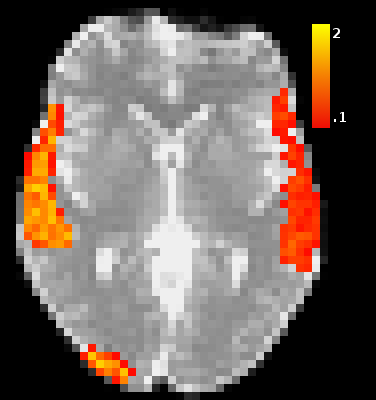
\includegraphics[width=\textwidth]{snr_hm.png}}
  \centerline{(a) SNR}\medskip
\end{minipage}
\hfill
\begin{minipage}[b]{.49\linewidth}
  \centering
  \centerline{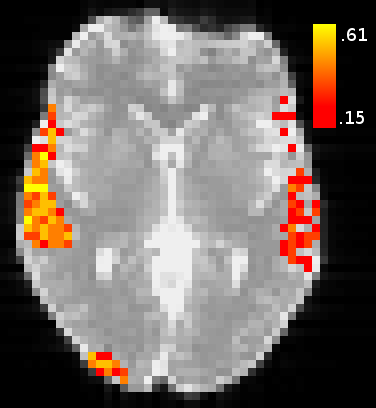
\includegraphics[width=\textwidth]{sim_hm_mi.png}}
  \centerline{(b) Mutual Information}\medskip
\end{minipage}
\caption{Results of POSSUM simulated data. $a)$ 
SNR of POSSUM additive noise. $b)$ Mutual Information between
the signal predicted by the particle filter and the actual signal.}
\label{fig:PossumResult}
\end{figure}

\begin{table}[t]
\ninept
  \centering
\begin{tabular}{| c | c | c | c | c | c |}
\hline
& Sim Value & \multicolumn{2}{|c|}{Prior} &\multicolumn{2}{|c|}{Posterior} \\
\hline
        &       &$\mu$  & $\sigma$& $\mu$& $\sigma$\\
\hline
$\tau_0  $& 1.45  & .98   & .25     & 1.07319 & 0.297749  \\
\rowcolor[gray]{.8} 
$\alpha  $&0.3    & .33   & .045    & 0.317955& 0.07311  \\
$E_0     $& 0.47  & .34   & .03     & 0.364195& 0.0457019  \\
\rowcolor[gray]{.8} 
$V_0     $& 0.044 & .04   & .03     & 0.110542& 0.0500039  \\
$\tau_s  $& 1.94  & 1.54  & .25     & 1.86785 & 0.390455  \\
\rowcolor[gray]{.8} 
$\tau_f  $& 1.99  & 2.46  & .25     & 2.50166 & 0.348326  \\
$\epsilon$& 1.8   & .7    & .6      & 1.58716 & 1.14536  \\
\hline
\end{tabular}
\caption{Comparison of the true value (left), the prior distribution
used to generate the initial particles (center two columns) and the 
average/variance of the estimates across simulated voxels. Note that
each voxel used the same underlying parameters (with differences only
in absolute value and noise realization), and all particle filters
were initialized with the same prior.}
\label{tab:beforeafter}
\end{table}[htb]

\section{Discussion}
\label{sec:Conclusion}
The data shows substantial correlation present in the parameter 
estimates for the 40 minute simulated data. Correlation of 
constants is a definite sign of the model being under-determined
and thus not observable. This is in spite of low noise, and the 
particle filter's solution converging to a Root-Mean-Squared error
of less than $0.002$. 

On a larger scale, the particle filter also performed well, clearly
locating regions of activation in spite of Signal-to-Noise Ratio 
well below 6dB. In spite of this, the final parameter estimates 
varied more than the initial (prior) distribution (\autoref{tab:beforeafter}).
This effect is slightly deceiving because the distributions
were far from Gaussian, and many were bi-modal. It is 
interesting, however, that such a wide range of solutions
could give good estimates for essentially one BOLD signal. 

From the results, it is clear that the BOLD model as presented
by Friston et al. is not observable, and thus parameter estimates
suffer from very large variance \cite{Friston2000}. As a result, parameter estimates
in that work are likely the result in the under-determination of
the model rather than underlying differences in parameters. 
There are two possible ways to deal with this problem. First, as
specified in Deneux et al., certain parameters could be locked into
place \cite{Deneux2006}. This solution is relatively easy, and would
also reduce computation time. True in-vivo parameter estimation
would help to determine proper values for parameters that are to be
kept constant, although it is a difficult proposition. The other
possible method is adding another measurement point. Technology exists
to simultaneously measure fMRI and \ac{CBF}. This additional
measurement, which is slightly closer to original stimulus, could
make the Balloon Model observable.

\small
\bibliographystyle{IEEEbib}
\bibliography{/home/micahc/library}

\end{document}
